\documentclass[hyperref={pdftex}]{beamer}
\usepackage{algorithm,algorithmic}
\useoutertheme{shadow}
\usetheme{Madrid}
% \addbibresource{references.bib}


\setbeamertemplate{section in toc}{\inserttocsectionnumber.~\inserttocsection}

\definecolor{mvablue}{rgb}{0.1098, 0.1373, 0.5137}
\definecolor{mvapurple}{rgb}{0.3373, 0.1529, 0.4510}
\definecolor{mvared}{rgb}{0.5725, 0.1882, 0.3922}

\colorlet{titleleft}{mvablue}
\colorlet{titlemiddle}{mvapurple}
\colorlet{titleright}{mvared}

\pgfdeclarehorizontalshading[titleleft,titlemiddle,titleright]
      {beamer@frametitleshade}{\paperheight}{
    color(0pt)=(titleleft);
    color(0.5\paperwidth)=(titlemiddle);
    color(\paperwidth)=(titleright)
  }

\useinnertheme{tcolorbox}
\addtobeamertemplate{title}{
  \begingroup
  \tcbset{
    enhanced,
    interior style={left color=mvablue,right color=mvared}
  }
}{\endgroup}

\title{Computational Statistics}
\subtitle{\textit{Hyperspherical VAE}}

\author{Victor Deng \and Inès Vati}
\institute[MVA]{École Normale Supérieure Paris-Saclay, Master MVA}
\date{$10^{\textrm{th}}$ JAN $2024$\\ \vspace{0.3cm} 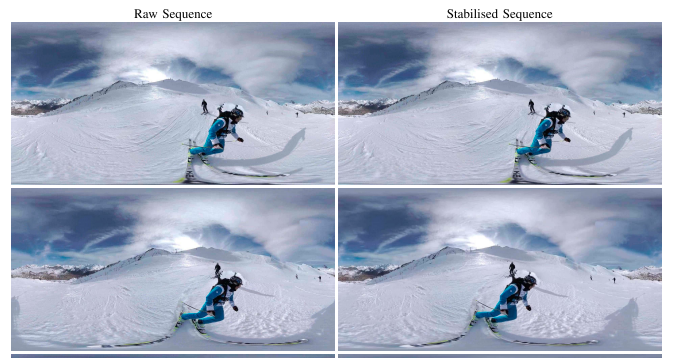
\includegraphics[scale=0.2]{figures/spherical_video.png}}

\logo{
\includegraphics[width=0.6cm]{figures/MVA-logo.png}}

\setbeamercolor{author in head/foot}{parent=palette primary,bg=}
\setbeamercolor{title in head/foot}{parent=palette secondary,bg=}

\makeatletter
\setbeamertemplate{footline}
{
    \leavevmode%
    \setbox\beamer@tempbox=\hbox{%
        \begin{beamercolorbox}[wd=.5\paperwidth,ht=2.25ex,dp=1ex,center]{author in head/foot}%
            \usebeamerfont{author in head/foot}\insertshortauthor\expandafter\beamer@ifempty\expandafter{\beamer@shortinstitute}{}{~~(\insertshortinstitute)}
        \end{beamercolorbox}%
        \begin{beamercolorbox}[wd=.5\paperwidth,ht=2.25ex,dp=1ex,center]{title in head/foot}%
            \usebeamerfont{title in head/foot}\insertshorttitle
        \end{beamercolorbox}%
        }%
        \beamer@tempdim=\ht\beamer@tempbox%
        \advance\beamer@tempdim by 4pt%
        \begin{pgfpicture}{0pt}{0pt}{\paperwidth}{10pt}
            \pgfpathrectangle{\pgfpointorigin}{\pgfpoint{\paperwidth}{\beamer@tempdim}}
            \pgfusepath{clip}
            \pgftext[left,base]{\pgfuseshading{beamer@frametitleshade}}
        \end{pgfpicture}
        \vskip-\beamer@tempdim%
        \box\beamer@tempbox%    
}%
\makeatother
  
\newcommand{\myitem}{\item[$\rightarrow$]}
\newcommand{\mycoolitem}{\item[\checkmark]}
\AtBeginSection[]
{
\begin{frame}{Table of contents}
\vfill
\tableofcontents[currentsection, hideallsubsections]
\vfill
\end{frame}
}

\begin{document}
\frame[plain]{\titlepage}

\begin{frame}
   \frametitle{Table of contents}
   \tableofcontents[subsectionstyle=hide]
\end{frame} 

\section{Introduction} 
\begin{frame}{Introduction}
    2018 paper from Tim R. Davidson \emph{et al.} \cite{davidson_hyperspherical_2022}
    \begin{itemize}
        \item Replacing the Gaussian prior and approximate posterior distributions with a von Mises-Fisher distribution
        \item Goal: better model data with a hyperspherical latent structure
        \item Various experiments, where the $\mathcal{S}$-VAE (von Mises-Fisher distributions) often outperforms the
        $\mathcal{N}$-VAE (Gaussian distributions) in low dimensions
    \end{itemize}
\end{frame}

\section{Sampling method}
\begin{frame}{Sampling $z'$ from vMF}
  \begin{algorithm}[H]
    \caption{Overview of the sampling method from $vMF(\mu, \kappa)$}\label{alg:overviewsampling}
    \begin{algorithmic}[1]
      \STATE Sample $z \sim q(z| e_1, \kappa)$ where $e_1 = (1, 0, \dots, 0)$
      \STATE Compute Householder reflection $U(\mu)$ so that $U(\mu) e_1 = \mu$
      \RETURN $z' = U(\mu) z$
    \end{algorithmic}
    \end{algorithm}
  \end{frame}

  \begin{frame}{Sampling $z$ from vMF}
    \begin{algorithm}[H]
      \caption{Overview of the sampling method from $vMF(\mu, \kappa)$}\label{alg:overviewsampling2}
      \begin{algorithmic}[1]
        \STATE Sample $z \sim q(z| e_1, \kappa)$ where $e_1 = (1, 0, \dots, 0)$
        \textcolor{red}{
          \STATE Sample $w \in \mathbb{R} \sim g(w |\kappa)$ by acceptance rejection sampling
          \STATE Sample $v \in \mathbb{R}^{d-1} \sim \mathcal{U}(S^{d-2})$ (uniform on the hypersphere $S^{d-2}$ independent of $w$)
          \STATE $z \gets (w, \sqrt{1 - w^2}v^T)^T$
        }
        \textcolor{gray}{
        \STATE Compute Householder reflection $U(\mu)$ so that $U(\mu) e_1 = \mu$
        \RETURN $z' = U(\mu) z \sim q(z' | \mu, \kappa)$}
      \end{algorithmic}
      \end{algorithm}
    \end{frame}
  
\begin{frame}{Sampling $w$ from $g(w|\kappa, \theta)$}
  \centering
  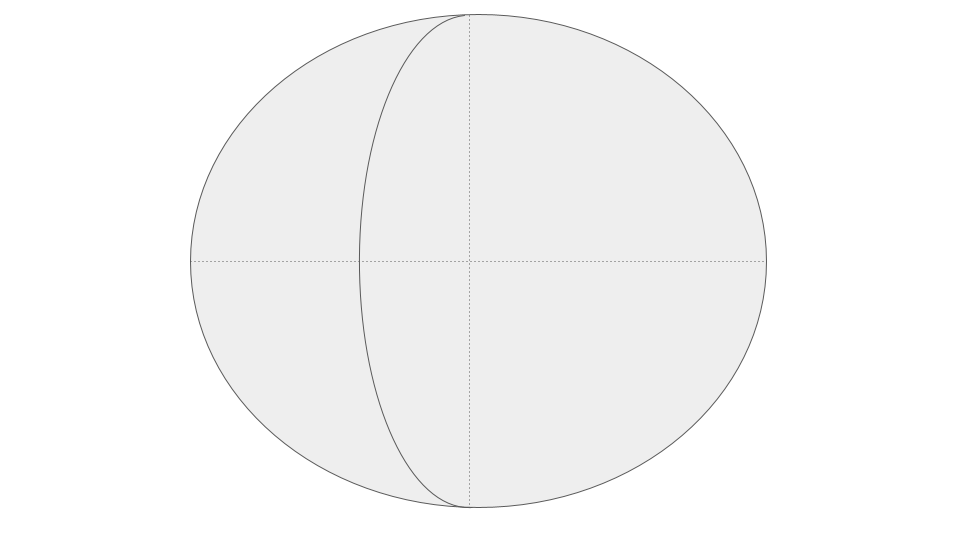
\includegraphics[width=\textwidth]{figures/illustration_sampling_1.png}
  $S^{2}$ : unit sphere in $\mathbb{R}^{3}$
\end{frame}

\begin{frame}{Sampling $w$ from $g(w|\kappa, \theta)$}
  \centering
  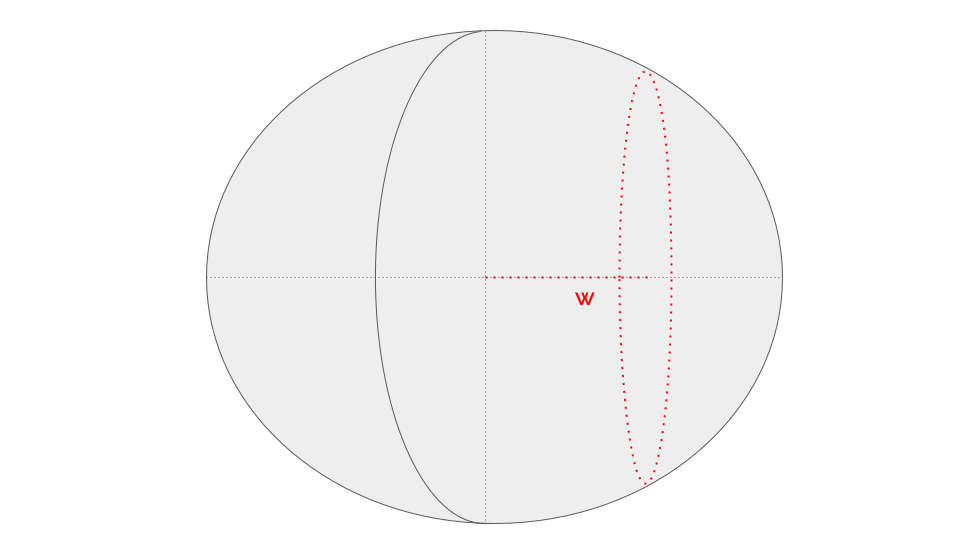
\includegraphics[width=\textwidth]{figures/illustration_sampling_2.png}  
  Sample $w \in \mathbb{R} \sim g(w |\kappa, d)$ by acceptance rejection sampling
\end{frame}

\begin{frame}{Sampling $w$ from $g(w|\kappa)$}
  \begin{itemize}
    \item[$\blacksquare$] Generale case
    \begin{itemize}
      \item Sample target distribution $w \in \mathbb{R} \sim g(w |\kappa)$ by sampling a proposal $w_{prop}$ of known density $r(w|\kappa)$
      \item Perform backpropagation by reparameterizing $r(w| \kappa)$ so that the sampling is independent of the parameters
      \item Note that $r$ is not explicitly given in the article
    \end{itemize}
  \end{itemize}
  \vfill
  \centering
  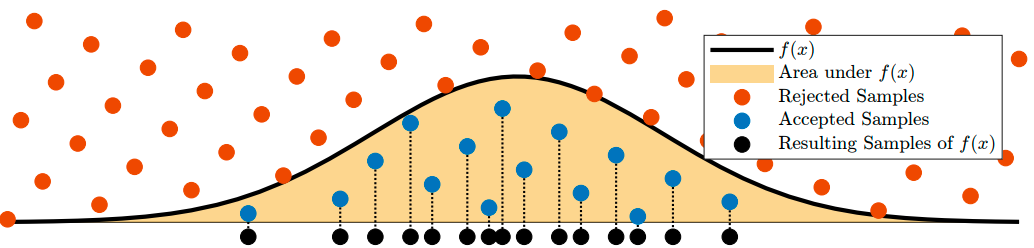
\includegraphics[height=.3\textheight]{figures/sampling_meth_illustration.png}
  \tiny{Illustration from \cite{frisch_rejection_2022}}
\end{frame}

\begin{frame}{Sampling $w$ from $g(w|\kappa)$}
  \begin{itemize}
    \item[$\blacksquare$] Case $d=3$ : faster to use inverse transformation method
    \begin{itemize}
      \item The vMF distribution explicity writes : $$ f_{vMF}(z) = \frac{\kappa}{4\pi\ sinh(\kappa)} exp(\kappa\mu^T z)  $$
      \item $(w, \sqrt{1 - w^2}v^T)^T \sim vMF(e_1, \kappa)$ where $v \sim \mathcal{S}^2$ and $w\in [-1, 1]$ has density $$ f_{W}(w) = \frac{\kappa}{2\ sinh(\kappa)} exp(\kappa w) $$
      \item We compute its cumulative distribution function $F_W(w)$ and its inverse  $$ F^{-1}_W (u) = \frac{1}{\kappa} ln(exp(-\kappa) + 2\ sinh(\kappa)u ) $$
      \item As $ sinh(\kappa) $ is numerically instable, we rewrites $$ F_W^{-1}(u) = 1 + \frac{1}{\kappa} ln(u + (1-u)exp(-2\kappa)) $$
    \end{itemize}
  \end{itemize}
\end{frame}

\begin{frame}{Sampling $v$ from $\mathcal{U}(S^{d-2})$}
  \centering
  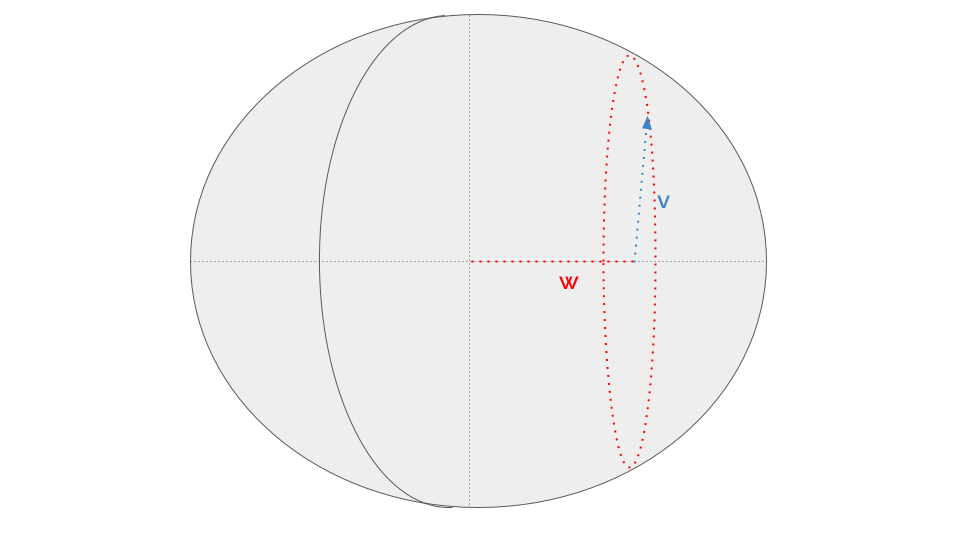
\includegraphics[width=\textwidth]{figures/illustration_sampling_3.png}
  \textcolor{blue}{Sample $v \in \mathbb{R}^{d-1} \sim \mathcal{U}(S^{d-2})$}
\end{frame}

\begin{frame}{Sampling $v$ from $\mathcal{U}(S^{d-2})$}
  \begin{itemize}
    \item $\mathcal{N}(0, I_{d-1})$ is rotationally symmetric around the origin
    \item $f_{Y_1, \dots, Y_{d-1}} = \frac{1}{\sqrt{2\pi}^{d-1}} exp(- (Y_1^2 + \dots + Y_{d-1}^2)/2) = \frac{1}{\sqrt{2\pi}^{d-1}}exp(-1^2/2) $ which is constant in all of the angular variables.
  \end{itemize}
  \vfill
  \begin{algorithm}[H]
    \caption{Sampling $v$ from $\mathcal{U}(S^{d-2})$}
  \begin{algorithmic}[1]
    \STATE Generate $d-1$ \textit{iid} variables $(X_i)$ from $\mathcal{N}(0, 1)$
    \STATE $Y_i \gets \frac{X_i}{\sqrt{X_1^1 + \dots + X_{d-1}^2}}$
    \RETURN $(Y_i)_{i=1, \dots, d-1} \sim \mathcal{U}(S^{d-2})$  
  \end{algorithmic}
  \end{algorithm}
\end{frame}

\begin{frame}{Sampling $z$ from $q(z|e_1, \kappa)$}
  \centering
  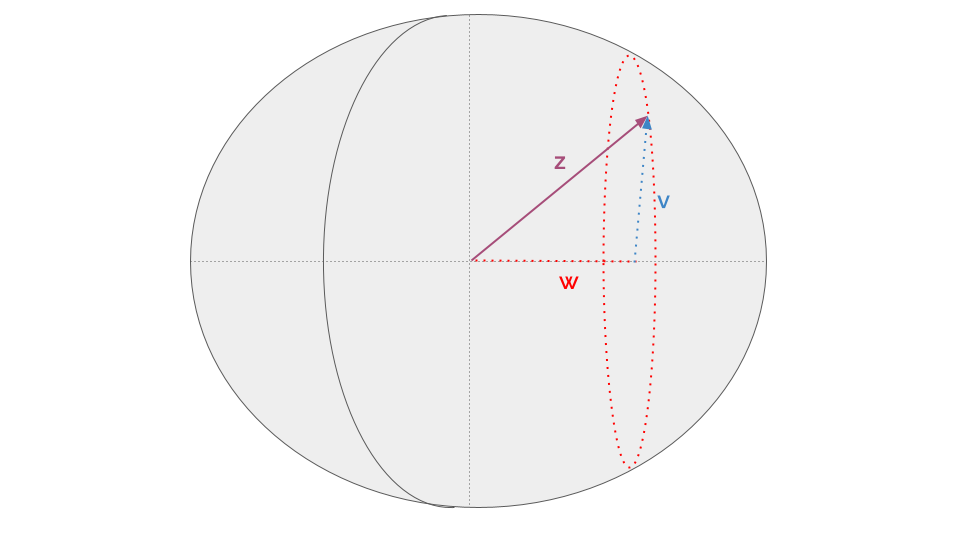
\includegraphics[width=\textwidth]{figures/illustration_sampling_4.png}
  \textcolor{magenta}{$z = (w, \sqrt{1 - w^2}v^T)^T$}
\end{frame}

\begin{frame}{Transform $z$}
  \begin{algorithm}[H]
    \caption{Overview of the sampling method from $vMF(\mu, \kappa)$}\label{alg:overviewsampling3}
    \begin{algorithmic}[1]
      \REQUIRE $\mu \in \mathbb{R}^d$, $\kappa \in \mathbb{R}_+$
      \textcolor{gray}{ \STATE Sample $z \sim q(z| e_1, \kappa)$ where $e_1 = (1, 0, \dots, 0)$ }
      \STATE Compute Householder reflection $U(\mu)$ so that $U(\mu) e_1 = \mu$
      \textcolor{red}{
      \STATE $u \gets Normalize(e_1 - \mu)$ 
      \STATE $U \gets I - 2uu^T$}
     \textcolor{red}{\RETURN $z' = U(\mu) z$}
    \end{algorithmic}
    \end{algorithm}
\end{frame}

\begin{frame}{Sampling results}
  \centering
  \begin{columns}
    \begin{column}{.5\textwidth}
      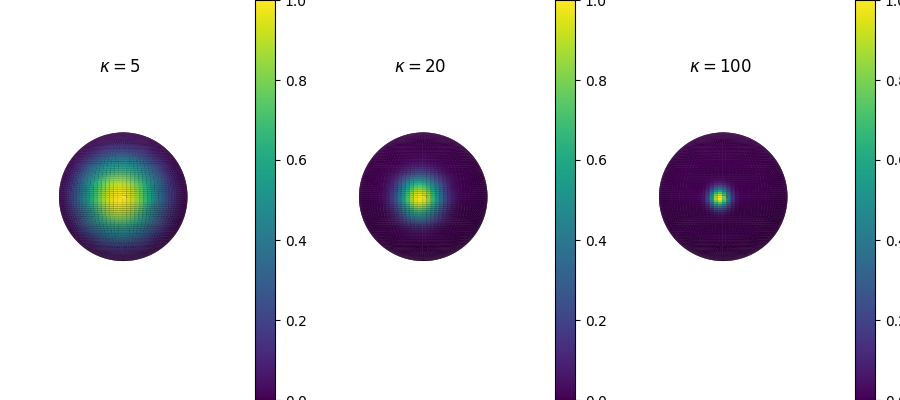
\includegraphics[width=\textwidth]{figures/vMF_density.png}
    \end{column}
    \begin{column}{.5\textwidth}
      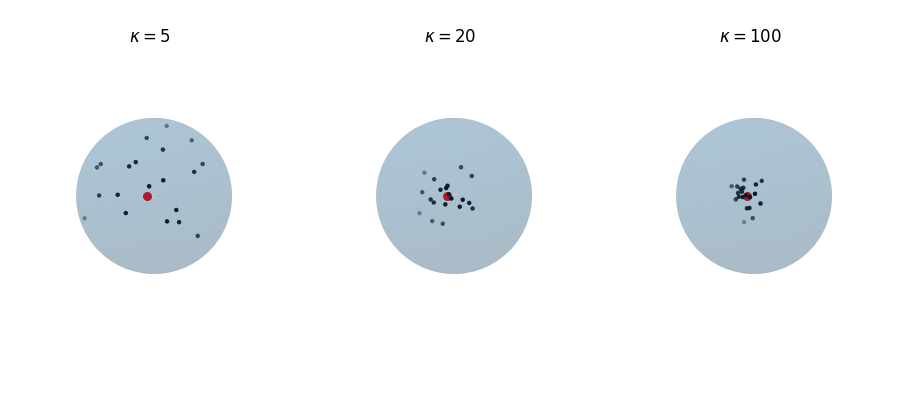
\includegraphics[width=\textwidth]{figures/vMF_sampling_ours.png}
    \end{column}
  \end{columns}
\end{frame}


\section{Reparameterization Trick}
\begin{frame}{Reparameterization Trick} % TODO Terminer
  The authors use a reparameterization trick that has been extended to distributions that can be sampled using rejection sampling \cite{naesseth2020reparameterization}.
  
  \begin{algorithm}[H]
    \caption{Reparameterized Rejection Sampling (from \cite{naesseth2020reparameterization})}\label{alg:rejectionsampling}
    \begin{algorithmic}[1]
    %\REQUIRE target $q(z; \theta)$, proposal $r(z; \theta)$, and constant $M_\theta$, with $q(z; \theta) \leq M_\theta r(z; \theta)$ 
    %\ENSURE $\varepsilon$ such that $h(\varepsilon,\theta) \sim q(z; \theta)$
    \STATE $i \gets 0$
    \REPEAT 
    \STATE $i \gets i +1 $
    \STATE Propose $\varepsilon_i \sim s(\varepsilon)$
    \STATE Simulate $u_i \sim \mathcal{U}[0,1]$
    \UNTIL $u_i < \frac{g\left(h(\varepsilon_i,\theta); \theta\right)}{r\left(h(\varepsilon_i,\theta) ; \theta\right)}$
    \RETURN $\varepsilon_i$
    \end{algorithmic}
    \end{algorithm}

  \end{frame}

% \begin{frame}{Monte Carlo estimates}
%   Estimating gradients with Monte Carlo estimates:
%   $$ \nabla_\theta \mathbb{E}_{g(\omega|\theta)}[f(\omega)] = \mathbb{E}_{\pi(\varepsilon|{\color{red}\theta})}[f(h(\varepsilon, \theta))] + \mathbb{E}_{\pi(\varepsilon|{\color{red}\theta})}\left[f(h(\varepsilon,\theta)) \nabla_\theta \log \frac{g(h(\varepsilon, \theta)|\theta)}{r(h(\varepsilon, \theta)|\theta)}\right] $$
%   Problem: the expectation is with respect to a distribution that depends on $\theta$.
  
%   No easy way to write it as $ \mathbb{E}[g(\theta, W)] $ with $W$ a random variable.

%   No reference to a convergence proof in \cite{davidson_hyperspherical_2022,naesseth2020reparameterization,paisley2012variational,mnih2014neural} 
%     %Regarder si la démonstration de la SGD marche même avec une espérance qui dépend de $\theta$ (reparameterization trick)
  
%   %Faire des expériences : échantillonnage d'une vMF, dataset Cora
  
% \end{frame}

\begin{frame}{Monte Carlo estimation}
  By noting $\pi(\varepsilon|\theta)$ the distribution of the resulting $\varepsilon$, we have (gradient of the expected log-likelihood)
  $$ \nabla_\theta \mathbb{E}_{g(\varepsilon|\theta)}[...] = \mathbb{E}_{\pi(\varepsilon|\theta)}[...] ~ {"}{=} ~ \mathbb{E}_{(\varepsilon_i, U_i)_i}[...]" $$
  \medskip

  % Similar to usual reparameterization trick (without rejection sampling), where
  % we compute Monte Carlo estimates of
  % $$ \nabla_\theta \mathbb{E}_{s(\varepsilon)}[f(h(\varepsilon, \theta), \theta)] $$
  % where $s(\varepsilon)$ is independent of $\theta$
  % \medskip

  Problem: $(\varepsilon_i, U_i)_{i \in \mathbb{N}}$ is not a random variable
  (it is a stochastic process)

  No reference to a convergence proof in \cite{davidson_hyperspherical_2022,naesseth2020reparameterization,paisley2012variational,mnih2014neural}
\end{frame}

\section{Experiments on link prediction}
\begin{frame}{Experiments on link prediction}

  \begin{itemize}
    \item Link prediction on a graph dataset: given a graph with some edges removed, predict the likelihood
    for each pair of nodes to be connected by an edge
    \item Cora dataset \cite{McCallum_2000}: 2708 publications, 5429 links, 1433-dimensional feature vectors
    \item Using a Variational Graph Auto-Encoder \cite{kipf_variational_2016}: a variational encoder which uses a
    graph neural network (GNN) as encoder
    \item Reconstruction loss:
        $$ \mathbb{E}_{q(\mathbf{Z}|\mathbf{X}, \mathbf{A})}(\log p(\mathbf{A}|\mathbf{Z})) \quad 
        \text{where} p(\mathbf{A}|\mathbf{Z}) = \prod_{i = 1}^N \prod_{j=1}^N p(A_{i, j}|\mathbf{z}_i, \mathbf{z}_j) $$
    \item Negative sampling: in the sum $\sum_{i, j} \log p(A_{i, j}|\mathbf{z}_i, \mathbf{z}_j)$, keep all
    positive edges and one randomly sampled negative edge per positive edge
  \end{itemize}
\end{frame}

\begin{frame}{TODO}

    reproduire l'experience 
  
    - \sout{data} (Ines)
  
    - \sout{implementer les modèles} (Victor VGAE)
    
    - gradients pour le hyperspherical VAE (Inès)
    
    - courbes d'entraînement dans le cas normal (Victor)
  
    - entrainement et evaluation 
  
  \end{frame}

  \begin{frame}{Loss computation}

    \begin{itemize}
      \item[$\blacksquare$] Reconstruction loss
        \begin{itemize}
          \item $$\mathcal{L}_{recon} =  - \mathbb{E}_{q_{\psi}}( log\ p_{\phi}(x | z)) $$
          \item$$ -\nabla_{\kappa} \mathcal{L}_{recon} \approx g_{recon} + g_{cor} $$ 
        \end{itemize}
      \item[$\blacksquare$] KL Divergence 
          \begin{itemize}
            \item $$ \mathcal{L}_{\mathcal{KL}} = \mathcal{KL}(q(z|\mu, \kappa) || p(z)) $$
            \item $$ \nabla_{\kappa} \mathcal{L}_{\mathcal{KL}} $$
          \end{itemize}
    \end{itemize}
    The formulas were explicity computed in the article.
    
  \end{frame}


\section{Conclusion and Discussion} 
\begin{frame}{Conclusion and Discussion}
  \begin{itemize}
    \item Quite meaningful contribution in low dimensions
    \item Algorithm not really useful in high dimensions, due to vanishing surface problem
    and soap bubble effect of the $\mathcal{N}$-VAE
    \item Much less variance parameters (1 vs. $d$ for $\mathcal{N}$-VAE), so possibly less expressivity
    \item vérifier différentes dimensions de l'espace latent 
    \item et algo vraiment utile en petite ou moyenne dimension ?
  \end{itemize}
  
  \end{frame}

\begin{frame}{References}
  \bibliographystyle{alpha} % Warning cite reference not with number but with name
  \bibliography{references}
\end{frame}

\end{document}